%%%%%%%%%%%%%%%%%%%%%%% file template.tex %%%%%%%%%%%%%%%%%%%%%%%%%
% $Id: woc_2col.tex 158 2017-01-19 23:08:23Z foley $
% $URL: https://repository.cs.ru.is/svn/template/tvd/journal/matec-woc/woc_2col.tex $
% 
% This is a template file for Web of Conferences Journal
%
% Copy it to a new file with a new name and use it as the basis
% for your article
%
% This template has been updated to match the Word Template's contents
% by Joseph T. Foley < foley AT RU dot IS >
%
%%%%%%%%%%%%%%%%%%%%%%%%%% EDP Science %%%%%%%%%%%%%%%%%%%%%%%%%%%%
%
%%%\documentclass[option]{webofc}
%%% "twocolumn" for typesetting an article in two columns format (default one column)
%
\documentclass[twocolumn]{webofc}
\usepackage[varg]{txfonts}   % Web of Conferences font
\usepackage{booktabs}
\usepackage{array} %% needed for advanced table manipulation
%% Column types from http://tex.stackexchange.com/questions/54069/table-with-text-wrapping
\newcolumntype{L}[1]{>{\raggedright\let\newline\\\arraybackslash\hspace{0pt}}m{#1}}
\newcolumntype{C}[1]{>{\centering\let\newline\\\arraybackslash\hspace{0pt}}m{#1}}
\newcolumntype{R}[1]{>{\raggedleft\let\newline\\\arraybackslash\hspace{0pt}}m{#1}}

\graphicspath{{graphics/}{graphics/arch/}{Graphics/}{./}} % Look in these folders for graphics
%
% Put here some packages required or/and some personnal commands
\usepackage{svg}
\usepackage{amsmath}
\usepackage{algorithm}
\usepackage{algpseudocode}
\usepackage{comment}
\usepackage{hyperref}
\usepackage{varioref}
%
%
\begin{document}
%
\title{Implementing Double DQN for Autonomous Control in Atari Video Pinball}
%
% subtitle is optionnal
%
%%%\subtitle{Do you have a subtitle?\\ If so, write it here}

\author{\firstname{Luca} \lastname{Mohr}\inst{1}\and
        \firstname{Christian} \lastname{Schmid}\inst{1}\and
        \firstname{Niklas} \lastname{Scholz}\inst{1}
        % etc.
      }

\institute{Baden-Wuerttemberg Cooperative State University Mannheim, Facility of economics, 68163 Coblitzallee 1-9, Germany
          }

\abstract{
In this paper, we present an approach to train an agent to play the Atari Video Pinball game using Deep Q-Networks (DQN), a popular reinforcement learning algorithm. DQN leverages deep learning to approximate Q-values, which represent the expected future rewards of taking actions in particular states. We preprocess the game frames, employ an epsilon-greedy strategy for action selection, and utilize a replay memory to store and sample experiences for training. Our results demonstrate the agent's capability to learn effective policies through iterative interaction with the game environment. We discuss the training process, challenges encountered, and potential improvements. This study contributes to the field of reinforcement learning by providing insights into the application of DQN in complex environments like Atari games.
%
  %You should leave 8 mm of space above the abstract and 10 mm after the abstract.
  %The heading Abstract should be typed in bold 9-point Times.
  %The body of the abstract should be typed in normal 9-point Arial in a single paragraph, immediately following the heading.
  %The text should be set to 1 line spacing.
  %The abstract should be centred across the page, indented 17 mm from the left and right page margins and justified.
  %It should not normally exceed 200 words.
}
%
\maketitle
%
\section{Introduction}\label{sec:page-layout}
The rapid advancement of reinforcement learning (RL), especially through the development and application of Deep Q-Networks (DQN). DQN is a prominent RL algorithm that utilizes deep learning techniques to approximate Q-values, which are critical for predicting the expected future rewards of taking specific actions in given states. This capability is essential for training agents to perform tasks that involve sequential decision-making and dynamic environments.

This paper presents an approach to train an agent to play the Atari Video Pinball game using the Double DQN algorithm. Atari games are renowned for their complexity and serve as a challenging benchmark for assessing the performance and robustness of RL algorithms. The methodology employed includes the preprocessing of game frames to provide the agent with meaningful input data, the implementation of an epsilon-greedy strategy to balance exploration and exploitation during action selection, and the utilization of a replay memory to store and sample experiences for effective training.

The experimental results demonstrate the agent’s capacity to learn effective policies through iterative interactions with the game environment. A detailed analysis of the training process, the challenges encountered, and potential improvements to enhance the agent’s performance is provided. 
\begin{comment}
The rapid advancement of artificial intelligence (AI) and machine learning (ML) has significantly propelled the field of reinforcement learning (RL), especially through the development and application of Deep Q-Networks (DQN). DQN is a prominent RL algorithm that utilises deep learning techniques to approximate Q-values, which are critical for predicting the expected future rewards of taking specific actions in given states. This capability is essential for training agents to perform tasks that involve sequential decision-making and dynamic environments.

\begin{figure}[!h]
\centering
\centerline{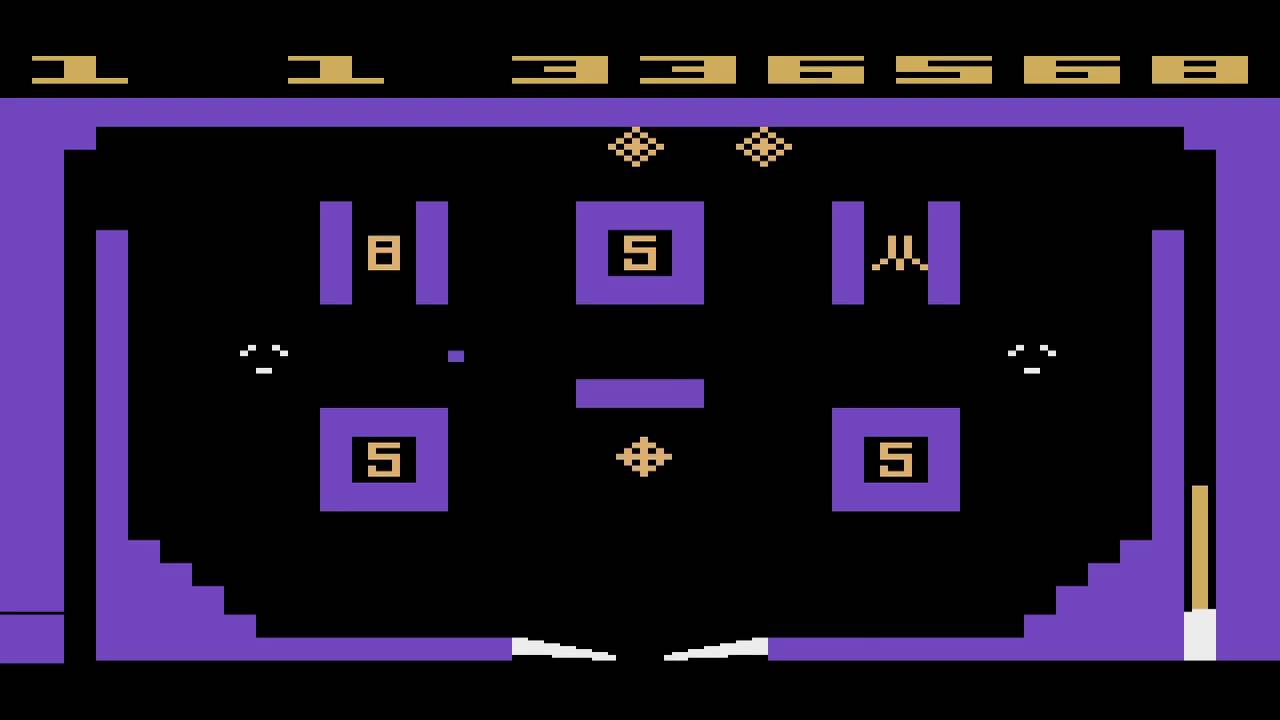
\includegraphics[scale=0.17]{graphics/game.jpg}}
\caption{This figure presents a demo of the actual game.}
\label{fig: game}
\end{figure} 

This paper presents an approach to train an agent to play the Atari Video Pinball game using the DQN algorithm. Atari games are renowned for their complexity and serve as a challenging benchmark for assessing the performance and robustness of RL algorithms. The methodology employed includes the preprocessing of game frames to provide the agent with meaningful input data, the implementation of an epsilon-greedy strategy to balance exploration and exploitation during action selection, and the utilisation of a replay memory to store and sample experiences for effective training.

The experimental results demonstrate the agent’s capacity to learn effective policies through iterative interactions with the game environment. A detailed analysis of the training process, the challenges encountered, and potential improvements to enhance the agent’s performance is provided. This study contributes to the field of reinforcement learning by offering insights into the practical application of DQN in complex environments such as Atari games. It thus advances our understanding of the algorithm’s strengths and limitations in real-world scenarios.
\end{comment}



\section{Related Work}

\subsection{Deep Q-Networks}

The work of Mnih et al. \cite{mnih2013playingatarideepreinforcement} led to the implementation of DQNs that successfully played Atari 2600 games, outperforming human experts in several games. The DQN architecture integrates a convolutional neural network (CNN) to approximate Q-values, and uses experience replay to reduce data correlation and stabilize the learning process. This methodology has been shown to be robust and effective, and has formed the basis for many subsequent studies in the field. A detailed explanation of how DQNs work, including the architecture and training process, is provided in subsection \ref{subsec: DQN}.

\subsection{Double DQN}
Several extensions of the original DQN algorithm have been developed to further improve its performance and stability. Double DQN, introduced by Van Hasselt et al. \cite{van_Hasselt_Guez_Silver_2016}, aims to reduce Q-value overestimation by using two separate networks, one for action selection and another for Q-value calculation.
%vorstellen in kapitel x.

\subsection{Experience Replay}
% Not uses in our paper
%Another notable extension is the Dueling DQN by Wang et al. \cite{pmlr-v48-wangf16}, which decomposes the Q-value function into two separate estimates: one for the benefit of a given action and another for the value of the state. This separation allows the agent to better evaluate the relative quality of actions in a given state, leading to faster and more stable learning.


%also not used in our paper, we use "normal distribution" experience replay
%\subsection{Prioritized Experience Replay}
%Schaul et al. \cite{schaul2016prioritizedexperiencereplay} introduced the concept of prioritised experience replay, where experiences are sampled based on their importance to learning rather than randomly. This technique improves training efficiency by ensuring that experiences that are more important and informative are replayed more often. 


% not relevant to our paper in my opinion
\begin{comment}
\subsection{Hierarchical Reinforcement Learning}
Another approach to enhancing the efficiency and scalability of RL is Hierarchical Reinforcement Learning (HRL). Dietterich \cite{dietterich2000hierarchical} introduced the MAXQ framework, which decomposes the learning task into a hierarchy of subtasks. This hierarchy helps the agent tackle complex tasks by breaking down the learning objectives into more manageable steps.
\end{comment}

\section{Contributions}
This paper extends the work of Mnih et al. \cite{mnih2013playingatarideepreinforcement} by implementing Double Deep Q-Networks (Double DQN) by Van Hasselt et al. \cite{van_Hasselt_Guez_Silver_2016}, which utilizes two separate networks for action selection and Q-value estimation. We then provide detailed analysis and insights into the training process, challenges encountered, and potential improvements.

\section{Atari Video Pinball Game}

\begin{figure}[!h]
\centering
\centerline{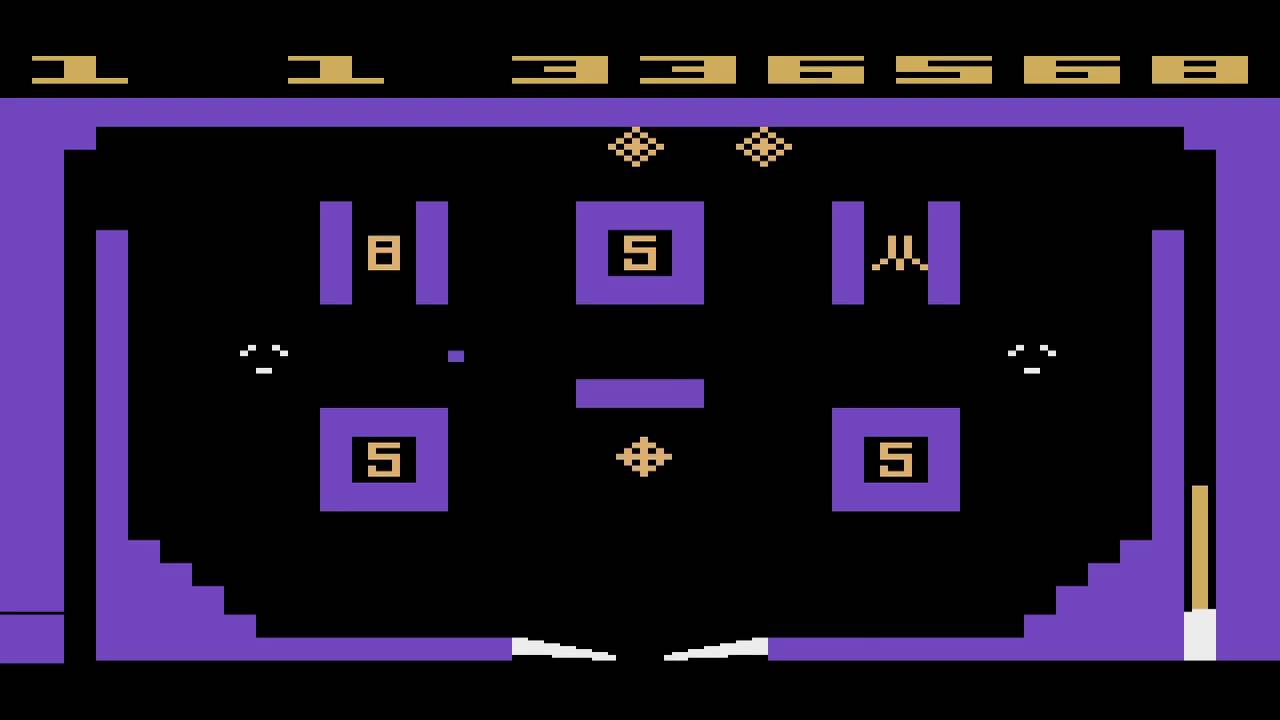
\includegraphics[scale=0.17]{graphics/game.jpg}}
\caption{This figure presents a demo of the actual game.}
\label{fig: game}
\end{figure}

"Atari Video Pinball", released by Atari, Inc. in 1980 for the Atari VCS (later known as the Atari 2600), is a video game that simulates the experience of playing a pinball machine. The game was developed by Bob Smith and incorporates essential elements of pinball, including flippers, bumpers, and a ball launcher. The player controls the aforementioned elements using the Atari joystick, thereby replicating the physical actions involved in traditional pinball gameplay. The movement of the joystick allows for the activation of the left and right flippers, while a downward pull on the joystick emulates the action of pulling back a plunger to launch the ball into play. \cite{newman2018atari}

The game is designed to emulate the dynamics of an arcade pinball machine, with digital enhancements. For example, the player is rewarded with an additional ball upon hitting the Atari logo on the playfield four times, thereby introducing an engaging element to the gameplay. Furthermore, the game incorporates features such as ball nudging, which enables players to subtly adjust the ball’s trajectory by holding down the joystick button and moving the controller. However, excessive nudging results in a state of tilt, which causes the ball to drain and simulates the response of a real pinball machine to excessive manipulation. \cite{newman2018atari}

Points are scored as follows: \cite{atari_videopinball}
\begin{itemize}
    \item SPINNERS: 1 point each time the ball hits the spinner.
    \item BUMPER: 100 times their current value. The value inside the bumper increases every time all of the diamond-shaped drop targets are knocked down.
    \item DROP TARGETS: 100 points each time a drop target is hit.
    \item ATARI ROLLOVER: 100 points; after hitting the ATARI rollover four times, you receive an extra ball. Each time it rolls over, the bonus multiplier increases by one. Only one extra ball can be awarded with each turn. The number of ATARI rollovers hit is indicated at the bottom of the screen by one Atari symbol for each hit.
    \item LEFT ROLLOVER: 100 points each time it rolls over. Its value increases by one with each hit. When the ball drains, you receive 1000 points for each time it has rolled over, up to 4000 points.
    \item SPECIAL LIT TARGET: This target lights up for only four seconds. It is located between the two lower bumpers. Each time it is hit, the screen flashes and you score 1000 points.
\end{itemize}

The bonus multiplier is tallied at the end of a turn.

This rapid scoring is accompanied with a "whirring" sound. When you have scored one million points, the score rolls over and starts again. When this happens, you do not lose the additional 999999 points; they remain part of your score. \cite{atari_videopinball}

The goal of the game is to achieve the highest possible score by skillfully using the flippers, nudging the ball, and hitting the various targets and bumpers on the playfield to maximize point accumulation and earn extra balls. This emulates the competitive and rewarding nature of traditional pinball gameplay, encouraging players to hone their reflexes and strategic planning. \cite{atari_videopinball}

%The gameplay mechanics of Atari Video Pinball entail a single-player mode in which players alternate control of the ball in order to achieve the highest possible score. The game's visual design and scoring system were innovative for their time, offering a digital representation of the physical pinball experience. It represents a notable example of early video game design, wherein developers sought to bring popular arcade experiences into the home environment. \cite{newman2018atari}

%In conclusion, "Atari Video Pinball" represents a notable early instance of video gaming that effectively translated the excitement and challenge of pinball into a home console format. The innovative use of the Atari joystick for game control and the engaging gameplay mechanics contribute to the significance of this title in the history of video gaming. \cite{newman2018atari}


\section{Methodology}
\subsection{Game Environment}
In our study, we utilized the ALE/VideoPinball-v5 environment from the Gymnasium library for training and evaluating our reinforcement learning models. This environment offers several advantages in terms of the richness of visual data and the ability to preprocess this data effectively for deep learning tasks. \cite{gymnasium}

\subsection{Configuration and Simplifications}
The ALE/VideoPinball-v5 environment produces RGB images as its primary output. These RGB frames provide a detailed visual representation of the game state, capturing all the graphical nuances and spatial information essential for the agent to understand the environment fully. We opted to use these RGB frames initially and then convert them to grayscale. Converting the frames to grayscale reduces computational complexity by eliminating color information, which is often redundant for the task, while still retaining the essential structural details. This approach balances the need for detailed visual information with computational efficiency, making it more effective than using the raw 128-byte RAM data, which is highly abstracted and lacks the rich context provided by image data. \cite{gymnasium}

For the action space, we used the Discrete(9) configuration, which includes nine possible actions the agent can take, displayed and explained in table \vref{tab:action_space}. This reduced action space simplifies the learning process by limiting the number of actions the agent must evaluate and choose from at each step. Using the full Discrete(18) action space, while providing a more granular control, significantly increases the complexity and computational burden of the learning process. By using Discrete(9), we strike a balance between providing the agent with sufficient action choices to perform effectively and maintaining a manageable level of complexity for our computational resources. \cite{gymnasium}



We employed the standard difficulty level for our experiments. The standard difficulty level provides a balanced challenge that allows for effective training and evaluation of the agent's capabilities. In contrast, the hard difficulty level increases the game's complexity, making it significantly more challenging for the agent to learn and perform well. Given the constraints of our computational resources, including the limited training epochs and inability to perform extensive hyperparameter optimization, the standard difficulty level was chosen to ensure the agent could achieve meaningful learning within these constraints. \cite{gymnasium} 

To streamline the training process and enhance computational efficiency, we utilized the standard frameskip setting of 4 in our experiments. This means that the environment repeats each selected action for 4 consecutive frames before allowing the agent to make a new decision. This frameskip approach reduces the frequency of action decisions, thereby lowering the computational load without significantly compromising the agent's ability to learn effective policies. By maintaining this standard frameskip, we ensure a balance between training efficiency and the quality of learned behaviors.

\begin{table}[!h]
\centering
\begin{tabular}{cl}
\toprule
\textbf{Value} & \textbf{Meaning} \\
\midrule
0 & NOOP: No operation, the \\
    & agent does nothing. \\ \addlinespace
1 & FIRE: Activates the fire \\
    & button, typically used \\
    & to launch the ball. \\ \addlinespace
2 & UP: Moves the paddle \\
    & or flipper up. \\ \addlinespace
3 & RIGHT: Moves the paddle \\
    & or flipper to the right. \\ \addlinespace
4 & LEFT: Moves the paddle \\
    & or flipper to the left. \\ \addlinespace
5 & DOWN: Moves the paddle \\
    & or flipper down. \\ \addlinespace
6 & UPFIRE: Moves the paddle \\
    & or flipper up while firing. \\ \addlinespace
7 & RIGHTFIRE: Moves the paddle \\
    & or flipper to the right \\
    & while firing. \\ \addlinespace
8 & LEFTFIRE: Moves the paddle \\
    & or flipper to the left \\
    & while firing. \\ \addlinespace
\bottomrule
\end{tabular}
\caption{Action space for VideoPinball on the Atari 2600. The table lists the discrete action values and their corresponding meanings.}
\label{tab:action_space}
\end{table}

 \label{subsec: config}
\subsection{Epsilon-Greedy-Method} \label{subsec: epsilon-greedy}
The $\epsilon$-greedy method represents a straightforward and prevalent approach to addressing the exploration-exploitation dilemma in reinforcement learning. It integrates two pivotal strategies: exploitation (the utilisation of current knowledge to maximise immediate benefits) and exploration (the investigation of novel actions with the objective of enhancing long-term outcomes). \cite{sutton-2018}
%\subsection{Functionality}

In the $\epsilon$-greedy procedure, the action with the highest estimated value is typically selected. However, a random action is selected with a small probability $\epsilon$. This random selection allows the agent to try out seemingly sub-optimal actions, which can lead to better insights in the long term.
The action $a_t$ in a given state $s_t$ is selected according to the following procedure \cite{sutton-2018}:
\begin{equation}
a_t =
  \begin{cases} 
   \text{argmax}_a Q(s_t, a) & \text{with probability } 1 - \epsilon \\
   \text{random action from $A$} & \text{with probability } \epsilon 
  \end{cases}
\end{equation}
The estimated reward for the action $a$ in state $s_t$ is given by $Q(s_t, a)$. The set of all possible actions is denoted by $A$.
The \textbf{advantages} of the $\epsilon$-greedy process are as follows. Firstly, the process guarantees exploration. Secondly, over time, each action is executed infinitely often, to ensure that all $Q(s_t, a)$ converge to their true values $q^*(s_t, a)$. \cite{sutton-2018} 

Thirdly, the method is simple to implement and does not require complicated calculations or models of the environment.\newline
One of the main \textbf{disadvantages} of the procedure is that it also selects suboptimal actions, which can lead to lower rewards in the short term. Additionally, the $\epsilon$-greedy process is non-adaptive. A constant value of $\epsilon$ can be suboptimal in different phases of the learning process. One way to improve this is to reduce the value of $\epsilon$ over time. \cite{sutton-2018}

%\subsection{Technical depth and formulas}


The $\epsilon$-greedy method is based on the estimation of the Q values, which can be adjusted by the following update step \cite{sutton-2018}:

\begin{equation}
    Q(s_t, a_t) \leftarrow Q(s_t, a_t) + \alpha [r_{t+1} + \gamma \max_a Q(s_{t+1}, a) - Q(s_t, a_t)]
\end{equation}

Here is:
The notation $Q(s_t, a_t)$ represents the current estimated value of the action $a_t$ in the state $s_t$. The notation $r_{t+1}$ denotes the reward received after performing $a_t$ in state $s_t$. The notation $\alpha$ represents the learning rate, while the notation $\gamma$ denotes the discount factor that devalues future rewards. \cite{sutton-2018}


\begin{comment}
\subsection{Practical effectiveness and applications}
In practice, the $\epsilon$-greedy method has been demonstrated to be effective, particularly in cases where the environment is stationary or only minor changes occur. It is particularly useful in the early stages of learning, when the agent still knows little about the environment and exploratory behaviour should be encouraged.
In applications such as display optimisation on web pages (e.g. personalised web services), the $\epsilon$-greedy method is employed to maximise both short-term clicks and to enhance long-term user interactions. \cite{sutton-2018}
\end{comment}

%\section{Deep Q-Network}
\subsection{Deep Q-Network} \label{subsec: DQN}
DQN represents an advance in RL through the integration of deep learning with Q-learning, enabling the handling of high-dimensional sensory inputs. This model is introduced by Mnih et al. \cite{mnih2013playingatarideepreinforcement} and represents the first successful framework that learns control policies directly from raw pixels using RL techniques. For example, DQN was applied to to Atari 2600 games in the Arcade Learning Environment (ALE) and demonstrated superior performance compared to to previous methods, achieving significant gains in six out of seven games and surpassing human experts in three. \cite{mnih2013playingatarideepreinforcement}

In the past, reinforcement learning with high-dimensional inputs such as speech was typically approached through the use of handcrafted features combined with linear value functions. However, these approaches were constrained by the quality of the feature representation. The significant advances in deep learning, particularly convolutional neural network (CNN) have enabled the extraction of high-level features from raw data, leading to notable success in computer vision and speech recognition. \cite{mnih2013playingatarideepreinforcement}

RL presents a number of distinctive challenges for deep learning, including the learning of sparse and noisy reward signals, the presence of high data correlation, and the necessity of dynamic data distributions. DQN addresses these challenges by integrating a CNN with a variant of the Q-learning algorithm and utilising experience replay to stabilise the training process. The agent interacts with the environment, selecting actions with the objective of maximising future rewards based on sequences of observed images. \cite{mnih2013playingatarideepreinforcement}

\subsubsection{Q-Learning} % TODO: Experience Replay besser erklären
The Q-learning algorithm updates the action-value function iteratively using the Bellman equation displayed in equation \ref{eq: bellman}, which is based on the following intuition: if the optimal value $Q(s', a')$ of the sequence $s'$ at the next time-step was known for all possible actions $a'$, then the optimal strategy is to select the action $a'$ maximizing the expected value of $r + \gamma Q(s', a')$: \cite{mnih2013playingatarideepreinforcement}

\begin{equation} \label{eq: bellman}
    Q(s, a) = \mathbb{E}_{s' \sim E} \left[ r + \gamma \max_{a'} Q(s', a') \mid s, a \right]
\end{equation}

A neural network function approximator, known as a Q-network, is used to estimate $Q(s, a; \theta) \approx Q^*(s, a)$, where $\theta$ represents the network weights. The network is trained by minimizing a sequence of loss functions $L_i(\theta_i)$, which measure the difference between predicted and target Q-values \cite{mnih2013playingatarideepreinforcement}, as shown in Equation \ref{eq: loss_function}.

\begin{equation} \label{eq: loss_function}
    L_i(\theta_i) = \mathbb{E}_{(s,a) \sim \rho(\cdot)} \left[ \left( y_i - Q(s, a; \theta_i) \right)^2 \right]
\end{equation}

where the target for iteration $i$ is given by equation \ref{eq: y_i}

\begin{equation} \label{eq: y_i}
    y_i = \mathbb{E}_{s' \sim E} \left[ r + \gamma \max_{a'} Q(s', a'; \theta_{i-1}) \mid s, a \right]
\end{equation}

The gradient of the loss function with respect to the weights is given by equation \ref{eq: gradient}.

\begin{equation}
\label{eq: gradient}
\begin{aligned}
\nabla_{\theta_i} L_i(\theta_i) = \mathbb{E}_{s, a \sim \rho(\cdot); s' \sim \mathcal{E}} \Bigg[ \left( r + \gamma \max_{a'} Q(s', a'; \theta_{i-1}) \right. \\
\left. - Q(s, a; \theta_i) \right) \nabla_{\theta_i} Q(s, a; \theta_i) \Bigg]
\end{aligned}
\end{equation}

\begin{comment}
\begin{equation}
    \nabla_{\theta_i} L_i(\theta_i) = \mathbb{E}_{(s,a) \sim \rho(\cdot); s' \sim E} \left[ \left( r + \gamma \max_{a'} Q(s', a'; \theta_{i-1}) - Q(s, a; \theta_i) \right) \nabla_{\theta_i} Q(s, a; \theta_i) \right]
\end{equation}
\end{comment}

% added epsilon greedy
DQN employs experience replay in order to address correlated data and non-stationary distributions. The algorithm employs a process of storing and randomly sampling the agent’s experiences, thereby enabling the reuse of experiences on multiple occasions. This approach serves to enhance the efficiency of the data and the stability of the learning process. The action is then sampled using the epsilon-greedy strategy, as described in subsection \ref{subsec: epsilon-greedy}. 
Combining Q-learning with neural networks, experience replay, and epsilon-greedy, we get an extension of the Q-learning algorithm, now called the Deep Q-learning algorithm, which can also be found as pseudo-code in Algorithm \ref{algo: deep_q_learning}.


\begin{algorithm}[H]
\caption{Deep Q-learning with Experience Replay}
\label{algo: deep_q_learning}
\begin{algorithmic}[1]
\State Initialize replay memory $\mathcal{D}$ to capacity $N$
\State Initialize action-value function $Q$ with random weights
\For{episode $= 1$ to $M$}
    \State Initialise sequence $s_1 = \{ x_1 \}$ and preprocessed \Statex \quad \quad sequence $\phi_1 = \phi(s_1)$
    \For{$t = 1$ to $T$}
        \State With probability $\epsilon$ select a random action $a_t$
        \State otherwise select $a_t = \arg\max_a Q^*(\phi(s_t), a; \theta)$
        \State Execute action $a_t$ in emulator and observe \Statex \quad \quad \quad reward $r_t$ and image $x_{t+1}$
        \State Set $s_{t+1} = s_t, a_t, x_{t+1}$ and \Statex \quad \quad \quad preprocess $\phi_{t+1} = \phi(s_{t+1})$
        \State Store transition $(\phi_t, a_t, r_t, \phi_{t+1})$ in $\mathcal{D}$
        \State Sample random minibatch of transitions \Statex \qquad \quad $(\phi_j, a_j, r_j, \phi_{j+1})$ from $\mathcal{D}$
        \State $y_j = \begin{cases} 
        r_j & \text{terminal } \phi_{j+1} \\
        r_j + \gamma \max_{a'} Q(\phi_{j+1}, a'; \theta) & \text{otherwise}
        \end{cases}$
        \State Perform a gradient descent step on \Statex \qquad \quad $(y_j - Q(\phi_j, a_j; \theta))^2$ according to equation 3
    \EndFor
\EndFor
\end{algorithmic}
\end{algorithm}
% TODO: Begründen, dass wir hier auf dem Paper aufgebaut haben mit dem 84 x 84 image
%The neural network processes the raw Atari frames, converting them to grayscale and downsampling them to an 84×84 image. The network comprises three hidden layers: two convolutional layers, followed by rectifiers, and a fully connected layer with 256 units. The output layer is responsible for predicting Q-values for all possible actions in a given state. \cite{mnih2013playingatarideepreinforcement}

\begin{comment}
The DQN algorithm was tested on seven Atari games: Beam Rider, Breakout, Enduro, Pong, Q*bert, Seaquest, and Space Invaders. In all seven games, the same architecture and hyperparameters were used. In order to limit the error scale, rewards were clipped. Furthermore, the RMSProp algorithm with minibatches of size $32$ was employed. The $\epsilon$-greedy policy strikes a balance between exploration and exploitation. The stability of the training process was demonstrated by the tracking of the average maximum predicted action-value function $Q$ throughout the training period. \cite{mnih2013playingatarideepreinforcement}
\end{comment}

\begin{comment}
The DQN method demonstrated superior performance to existing RL methods and human experts on several games, indicating its capacity to learn directly from raw inputs without prior knowledge. The advent of DQNs represents a pivotal moment in the integration of deep learning and reinforcement learning. By effectively merging Q-learning with deep convolutional neural networks (CNNs) and experience replay, this approach has set a new standard for reinforcement learning (RL) algorithms, achieving state-of-the-art results on a variety of Atari games. This success serves to illustrate the potential of deep learning techniques in addressing complex RL tasks, thereby paving the way for future advancements in the field. \cite{mnih2013playingatarideepreinforcement}
\end{comment}

% \begin{equation}
% Q(S_t, A_t) \leftarrow Q(S_t, A_t) + \alpha \left[ R_{t+1} + \gamma \max_a Q(S_{t+1}, a) - Q(S_t, A_t) \right].
% \end{equation}



%\vspace{1.5\baselineskip}
%\section{Implementation}


\subsubsection{Double Deep Q-Networks}
\label{subsec:double_dqn}
To address the overestimation bias present in standard DQNs, we implement Double Deep Q-Networks (Double DQN) as introduced by van Hasselt et al. \cite{van_Hasselt_Guez_Silver_2016}. Double DQN utilizes two separate networks: a policy network and a target network. The policy network selects actions, while the target network estimates the Q-values. This separation helps to reduce the overestimation bias.

In Double DQN, the Q-value update rule is modified to use the action selected by the policy network for the Q-value estimation by the target network, which can be represented as equation \ref{eq: double-DQN}

\begin{equation} \label{eq: double-DQN}
y = r + \gamma Q_{\text{target}}(s', \text{argmax}_{a'} Q_{\text{policy}}(s', a'))
\end{equation}

where $Q_{\text{target}}$ and $Q_{\text{policy}}$ denote the Q-values estimated by the target and policy networks, respectively. This approach decouples the action selection from the Q-value estimation, effectively reducing overestimation bias.

The target network's weights are periodically updated with the policy network's weights to ensure stability in learning. The use of two networks allows for more accurate Q-value estimates and leads to improved learning stability and performance.

\subsection{Implementation}
%\subsection{Baseline}
\subsubsection{Baseline}

The initial phase of the baseline method involves executing a specific sequence of actions designed to ensure the ball enters the playfield.

Following this introductory sequence, the Agent continues to trigger both flippers continuously. This approach embodies a naive "spam" strategy, similar to the behavior one might expect from a child repeatedly pressing the same button. The rationale for this method is twofold. First, it simulates a simplistic and unsophisticated play style, thereby establishing a minimal performance benchmark. Second, it is computationally efficient since the action does not require complex calculations but rather involves executing the same command repeatedly.

The episode concludes based on the game’s standard termination signals or a custom condition that checks for the ball being stuck. If the ball's position remains unchanged for 30,000 frames (approximately 5 seconds), the episode terminates to prevent prolonged inactivity.

This baseline was evaluated over three epochs, with the cumulative score recorded for each episode. The mean score across these epochs serves as the benchmark for future comparison. The simplicity and reproducibility of this baseline make it an ideal starting point for further experimentation. Moreover, it provides a clear, quantifiable measure against which more advanced, sophisticated models can be assessed.

%\subsection{Preprocessing}
\subsubsection{Preprocessing}
To reduce the computational costs associated with processing frames of \(210 \times 160\) pixels and a 128-color palette that the Atari environment returns, the frames were first converted from RGB to greyscale and then cropped to \(84 \times 84\) pixels. This preprocessing step significantly reduces the dimensionality of the input data, thereby decreasing computational complexity and memory usage. 

Additionally, four consecutive frames were stacked together to form the input to the Deep Q-Network (DQN). This stacking of frames captures the temporal dynamics of the game environment, allowing the network to understand motion and predict future states based on past observations. By providing a sequence of frames as input, the DQN can learn more complex behaviors and strategies by comprehending how the game evolves over time.

The optimal action is then determined based on the stacked frames and applied uniformly over 4 frames as mentioned in subsection \ref{subsec: config}. This approach reduces computational effort by minimizing the frequency of action selection while maintaining the temporal coherence necessary for effective decision-making in the game environment.
%\subsection{Network architecture}
\subsubsection{Network architecture}
\begin{comment}
\begin{figure}[!h]

\includesvg[scale=0.19]{graphics/nn-3.svg}
\caption{Architecture of the concolutional layers}
\label{fig: CNN}
\end{figure}

The network architecture comprises three convolutional layers, each followed by a batch normalization layer to stabilize and accelerate the training process by reducing internal covariate shift \cite{ioffe2015batch}. The detailed configuration of these layers is as follows: The first convolutional layer takes four input channels, corresponding to stacked frames, and outputs 32 channels using an $8\times8$ kernel with a stride of 4. This layer is responsible for capturing coarse spatial features from the input frames. The output is then normalized by the first batch normalization layer. The second convolutional layer takes 32 input channels and outputs 64 channels using a $4\times4$ kernel with a stride of 2. This layer further refines the spatial details and patterns extracted by the first layer, and its output is normalized by the second batch normalization layer. The third convolutional layer takes 64 input channels and outputs 64 channels using a $3\times3$ kernel with a stride of 1. This layer focuses on extracting fine-grained features from the previously processed feature maps, and its output is normalized by the third batch normalization layer. Each convolutional layer utilizes the ReLU activation function, introducing non-linearity into the model and enabling it to learn complex patterns. \cite{nair2010rectified}

Following the convolutional and normalization layers, the feature maps are flattened and passed through a fully connected layer. The input to this layer is calculated as the product of the height, width, and number of channels of the final feature maps, resulting in a feature vector that feeds into the fully connected layer. The input size is determined by the dimensions of the feature maps after the last convolutional layer. This layer outputs the Q-values for each of the 9 possible actions, representing the expected future rewards for taking each action from the current state. Thus, the output size is 9. During the forward pass, the input tensor, which consists of a stack of four consecutive frames, undergoes the following transformations: convolution, batch normalization, and ReLU activation in the first layer; convolution, batch normalization, and ReLU activation in the second layer; convolution, batch normalization, and ReLU activation in the third layer; flattening of the feature maps; and finally, processing through the fully connected layer to produce the Q-values. Importantly, this architecture allows for the computation of Q-values for all 9 possible actions with a single forward pass through the network.
\end{comment}
\begin{figure}[!h]
\includesvg[scale=0.19]{graphics/nn-3.svg}
\caption{Architecture of the convolutional layers}
\label{fig: CNN}
\end{figure}

The network architecture for the policy and target networks consists of three convolutional layers, which are visualized in figure \ref{fig: CNN}, each followed by a batch normalization layer to stabilize and accelerate training by reducing internal covariate shift \cite{ioffe2015batch}, and a fully connected layer afterwards to predict the actual Q-values. This architecture is inspired by the design proposed by Mnih et al. \cite{mnih2013playingatarideepreinforcement}, which has been proven effective in various reinforcement learning tasks. The first convolutional layer, with four input channels for stacked frames, outputs 32 channels using an $8\times8$ kernel with a stride of 4, capturing coarse spatial features. The second convolutional layer outputs 64 channels from 32 input channels using a $4\times4$ kernel with a stride of 2, refining spatial details and patterns. The third convolutional layer further processes the 64 input channels into 64 output channels using a $3\times3$ kernel with a stride of 1, extracting fine-grained features. Each convolutional layer uses the ReLU activation function to introduce non-linearity, enabling the model to learn complex patterns \cite{nair2010rectified}.

Following the convolutional and batch normalization layers, the feature maps are flattened into a vector with a size of 3136, calculated as $7\times7\times64$ based on the dimensions of the final feature maps. This vector serves as input to a fully connected layer. This fully connected layer outputs Q-values for the 9 possible actions, representing the expected future rewards for each action from the current state. Thus, the output size is 9. During the forward pass, the input tensor (a stack of four consecutive frames) undergoes sequential transformations: convolution, batch normalization, and ReLU activation in each of the three convolutional layers, followed by flattening and processing through the fully connected layer to produce the Q-values. This architecture enables the computation of Q-values for all 9 actions with a single forward pass.

%\subsection{Training and Optimization}
\subsubsection{Training and Optimization}
The training process leverages a replay memory to store experiences in the form of (state, action, next\_state, reward) tuples. The replay memory has a capacity of 50,000, allowing it to retain a significant history of the agent's interactions with the environment. These experiences are sampled randomly in batches of 128 to break the temporal correlations and are used to train the network, which stabilizes the learning process. Various batch sizes (32, 64, 128, 256) were tested, and it was observed that a batch size of 128 resulted in the best performance in terms of minimal loss and time taken, as shown in the respective table \ref{tab: batch sizes}. This method ensures that the distribution of experiences used for learning better represents the true environment dynamics, thereby enhancing the stability and efficiency of the training. The optimization of the network parameters is done using the AdamW optimizer with a learning rate of $1 \times 10^{-4}$, which helps in mitigating the issues of vanishing and exploding gradients.

\begin{table}[!h]
    \centering
    \begin{tabular}{rrr}
        \toprule
         \textbf{batch size} & \textbf{average loss per epoch} & \textbf{time taken} 
         \\ \midrule
          32 & 5.58  & 119.43s \\ \addlinespace
         64 & 5.93 & 172.96s \\ \addlinespace
        128 & 4.37 & 93.42s \\ \addlinespace
         256 & 4.54 & 168.93s \\ \addlinespace
         \bottomrule
    \end{tabular}
    \caption{The table illustrates the average loss over ten epochs and the time taken for different batch sizes. A batch size of 128 achieves the lowest average loss of 4.37 with the shortest training time of 93.42 seconds, indicating optimal performance and efficiency. In contrast, increasing the batch size to 256 results in a slightly higher average loss of 4.54 and a significantly longer training time of 168.93 seconds, highlighting the trade-off between batch size and computational load. Smaller batch sizes, such as 32 and 64, exhibit higher average losses and longer training times compared to the optimal batch size of 128.}
    \label{tab: batch sizes}
\end{table}

A target network is used alongside the policy network to compute the target Q-values. The weights of the target network are updated periodically using a soft update mechanism controlled by the parameter $\tau = 0.005$. This approach prevents the oscillations and divergence often observed when the policy network is directly used to estimate the target Q-values. \cite{mnih2013playingatarideepreinforcement}

The loss function used is Smooth L1 Loss, which is less sensitive to outliers compared to the mean squared error loss \cite{hastie-2009}.
This choice is crucial for stabilizing the training process, as it balances the robustness and sensitivity required for accurate Q-value estimation.


DQN agents were trained over a total of 500 epochs, with each epoch comprising 3 episodes, resulting in a cumulative training set of 1500 episodes. Throughout the training process, key performance metrics were recorded at the end of each epoch. These metrics included the average reward per epoch, the average duration per epoch, the loss values, and the epsilon decay. Epsilon decay follows an exponential decay rule, defined as in equation \ref{eq: epsilon_decay}

\begin{equation} \label{eq: epsilon_decay}
\epsilon = \epsilon_{\text{end}} + (\epsilon_{\text{start}} - \epsilon_{\text{end}}) \times \exp\left(-\frac{\text{steps\_done}}{\epsilon_{\text{decay}}}\right),
\end{equation}

where \(\epsilon_{\text{start}} = 0.9\), \(\epsilon_{\text{end}} = 0.05\), and \(\epsilon_{\text{decay}} = 1000\). This rule ensures a gradual transition from exploration to exploitation as training progresses. Post-training, these metrics were plotted to visualize the agent's learning progress and performance trends. The resulting graphs are presented in Figures \ref{fig: episode_duration} through \ref{fig: loss}.

Figure \ref{fig: episode_duration} illustrates the duration of each epoch, with initial high variability and significant spikes that stabilize over time, indicating improved training efficiency. In Figure \ref{fig: episode_reward}, the reward per epoch is shown, where initial high variability and significant peaks gradually decrease as the model converges, highlighting the learning process. The epsilon decay over training steps is presented in Figure \ref{fig: epsilon_decay}, demonstrating the transition from exploration to exploitation, which is essential for the model's convergence. Finally, Figure \ref{fig: loss} displays the loss values over optimization steps, reflecting the model's learning process with high initial variability and more stable periods indicating convergence phases.


\begin{figure}[!h]
\centering
\includesvg[scale=0.4]{graphics/epoch_duration.svg}
\caption{Epoch duration plot during the training of the policy network (DQN). The x-axis represents the epoch number, and the y-axis shows the duration in seconds. The blue line shows the raw duration per epoch, and the orange line is the moving average of the last 50 epochs. Initial high variability and significant spikes suggest initial inefficiencies, which stabilize over time. The moving average smooths short-term fluctuations, highlighting longer-term trends essential for diagnosing and optimizing training performance.}


\label{fig: episode_duration}
\end{figure}

\begin{figure}[!h]
\centering
\centerline{\includesvg[scale=0.4]{graphics/epoch_reward.svg}}
\caption{Epoch reward plot during the training of the policy network (DQN). The x-axis represents the epoch number, and the y-axis shows the reward. The blue line indicates the raw reward per epoch, while the orange line represents the moving average of the rewards. The plot shows initial high variability in rewards with significant peaks, which gradually decrease as training progresses. This pattern indicates the learning process of the model, with early exploration leading to high variability and later stabilization as the model converges. The moving average line smooths out short-term fluctuations and highlights longer-term trends, aiding in evaluating and optimizing the training performance.}
\label{fig: episode_reward}
\end{figure}

\begin{figure}[!h]
\centering
\centerline{\includesvg[scale=0.4]{graphics/epsilon_decay.svg}}
\caption{Epsilon decay plot during the training of the policy network (DQN). The x-axis represents the training step number, and the y-axis shows the epsilon value. The blue line indicates the decay of the epsilon value over time, reflecting the transition from exploration to exploitation. Initially, the epsilon value is high, promoting exploration of the action space. As training progresses, epsilon decays exponentially, reducing the exploration rate and increasing reliance on the learned policy. This decay helps balance exploration and exploitation, which is crucial for the convergence and performance of the DQN.}
\label{fig: epsilon_decay}
\end{figure}

\begin{figure}[!h]
\centering
\centerline{\includesvg[scale=0.4]{graphics/loss.svg}}
\caption{Loss plot during the training of the policy network (DQN). The x-axis represents the optimization step, while the y-axis shows the loss value. The blue line indicates the loss at each optimization step. The plot shows the fluctuations in the loss during training, reflecting the model's learning process. High initial variability in loss suggests the network's adjustments to the training data, with more stable periods indicating convergence phases. Monitoring the loss over time helps in diagnosing training issues, assessing model performance, and ensuring effective convergence of the deep Q-learning model.}
\label{fig: loss}
\end{figure}


%\subsection{Comparison}
%\subsection{Comparison}
\section{Comparison}
Lastly, the performance of the baseline method and the final model was compared. For this comparison, both models were evaluated over 10 epochs. The results of this comparison are presented in Table \ref{tab: results}. This table visualizes the rewards obtained by each model, providing a clear depiction of their respective performances. The comparison underscores the significant improvement achieved by the final model over the baseline.


Figure \ref{fig: q-values} illustrates the predicted Q-values over a sequence of 150 frames, beginning from frame 50, to capture the game's dynamics during mid-game rather than at the start. Within this interval, Frame 19 exhibits the lowest Q-value, close to zero, indicating minimal expected future rewards. As shown in Figure \ref{fig: frame19}, corresponding to Frame 19, the ball is positioned on the right side of the screen, isolated from any nearby targets that could be struck in subsequent frames to accumulate points. This observation aligns with the low Q-value, reflecting the anticipation of limited future rewards.

Conversely, Frame 54 in Figure \ref{fig: frame54} shows the highest Q-value, suggesting substantial expected future rewards. Examining the corresponding Frame 54 in Figure z reveals the ball poised to hit a target, which would result in scoring points. This is corroborated by the significant increase in the current score to 1500, compared to the score of 100 in Frame 19. Additionally, the inversion of colors from black to white indicates a noteworthy event, in this case, the ball striking the target. These observations substantiate the high Q-value's implication of considerable future rewards, validating the model's predictive accuracy.
%Figure x shows the predicted Q-values over the time for 150 frames, starting from frame 50 that we have a look at the frames during mid game and not directly at the beginning. In this Zeitraum, Frame 19 has the lowest Q-value of nearly 0, that indicitates low future rewards. If we have a look at figure y, that represents the corresponding frame 19, we see the ball on the right of the screen without having any targets in the umgebung that he could hit in the next few frames to score some points, which confirms the hypothesis of low future rewards refelcting the low Q-value. On the other hand, frame 54 in the figure x has the highest q-value indicating high future rewards. Looking at the corresponding frame, displayed in figure z, we can see that the ball is in the moment to hit the target and gain some points. This hypothesis is also confirmed by the current score of 1500 that is much higher than the score of 100 in frame 19. Also the color invertion of black into white signalises, that something special has happened, in this case the ball hits at exactly this moment the target. These impressions confirm the hypothesis of high future rewards derived by the high q-value in figure x. 

\begin{figure}
    \centering
    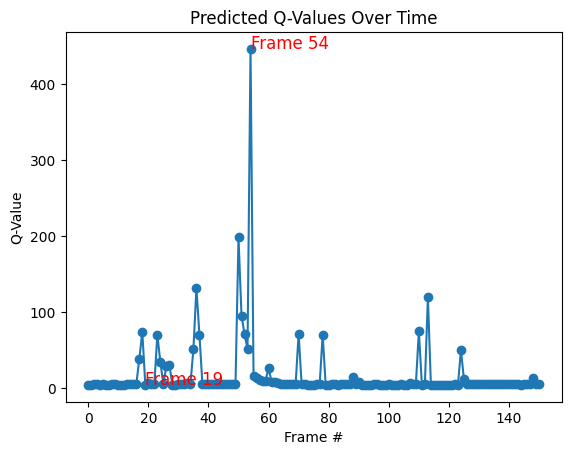
\includegraphics[width=0.8\linewidth]{graphics/q-values.png}
    \caption{The plot illustrates the predicted Q-values over a sequence of 150 frames, beginning from frame 50 and skipping the initial 50 frames to focus on the mid-game segment. The x-axis represents the frame number, while the y-axis shows the Q-value, indicating the expected future reward for the best action taken from that frame. The highest Q-value occurs at Frame 54, suggesting a significant positive event or reward, while the lowest Q-value is observed at Frame 19, potentially indicating a less favorable state or an immediate negative outcome. The significant fluctuations in Q-values highlight critical decision points and the agent's varying confidence levels throughout the game sequence, providing insights into the agent's decision-making process during mid-game play.}
    \label{fig: q-values}
\end{figure}

\begin{figure}
    \centering
    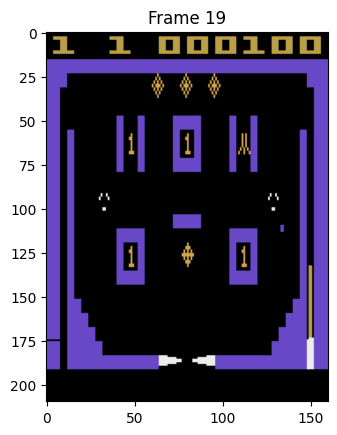
\includegraphics[width=0.7\linewidth]{graphics/frame19.png}
    \caption{The figure shows the 19th frame of the game. The ball is positioned on the right side of the screen, isolated from any nearby targets that could be struck in subsequent frames to accumulate points. This observation aligns with the low Q-value, reflecting the anticipation of limited future rewards.}
    \label{fig: frame19}
\end{figure}

\begin{figure}
    \centering
    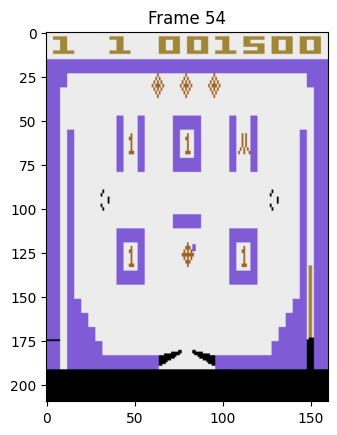
\includegraphics[width=0.7\linewidth]{graphics/frame54.png}
    \caption{Frame 54 shows the frame of the highest Q-value, suggesting substantial expected future rewards. The ball is poised to hit a target, which would result in scoring points. This is corroborated by the significant increase in the current score to 1500, compared to the score of 100 in Frame 19. Additionally, the inversion of colors from black to white indicates a noteworthy event, in this case, the ball striking the target. These observations substantiate the high Q-value's implication of considerable future rewards, validating the model's predictive accuracy.}
    \label{fig: frame54}
\end{figure}




\begin{table}[!h]
    \centering
    \begin{tabular}{lr}
        \toprule
         \textbf{Model} & \textbf{Average Reward per Epoch} 
         \\ \midrule
         Baseline & 2931.6  \\ \addlinespace
         DQN & 12078.8 \\ \addlinespace
         \bottomrule
    \end{tabular}
    \caption{Comparison of average rewards per epoch for baseline and DQN models in the Atari Video Pinball environment. The DQN model significantly outperforms the baseline model, achieving a substantially higher average reward per epoch. These models were compared over 5 epochs, which resulted in a total of 15 episodes.}
    \label{tab: results}
\end{table}


\section{Discussion and future work}
The preprocessing steps implemented, including converting frames to greyscale, cropping to \(84 \times 84\) pixels, and stacking four consecutive frames, have significantly reduced computational costs and improved training efficiency for the Atari Video Pinball environment. However, several limitations are inherent to this approach.

Converting frames to greyscale may lead to the loss of valuable color information that could potentially aid in the game's decision-making process. For instance, certain visual cues that rely on color differentiation are lost, potentially impacting the agent's ability to make informed decisions.

The fixed cropping to \(84 \times 84\) pixels, while reducing dimensionality, may exclude critical parts of the game environment. In Atari Video Pinball, where the entire playing field and paddle positions are essential, this fixed cropping might omit relevant areas, impacting the agent's performance.

Moreover, while stacking four frames helps capture temporal dynamics, it is a simplistic method that may not fully represent the intricate temporal dependencies present in the game. The fixed frame stack size introduces a hyperparameter that requires careful tuning, which was not extensively optimized due to limited computational resources.

Training the model effectively necessitated the use of GPU resources, which were not available locally. Consequently, we utilized Google Colab's NVIDIA TESLA T4 GPU for our computations, but the available resources were constrained by time limits. This constraint necessitated limiting the training to only 500 epochs and precluded extensive hyperparameter tuning, such as grid search. Only the batch size was varied and benchmarked in a brief trial, which may not have identified the optimal hyperparameters for the best performance.



Future research should focus on addressing these limitations to enhance the performance and efficiency of deep reinforcement learning models for Atari Video Pinball. One potential direction is to explore techniques that selectively incorporate color information, allowing the model to leverage both greyscale and color data where beneficial. 

Adaptive cropping methods could dynamically focus on the most relevant regions of each frame, ensuring that critical areas are retained and important contextual information is preserved. These methods could involve attention mechanisms or saliency detection to identify and prioritize crucial parts of the game environment.

To better capture temporal dependencies, employing more sophisticated architectures such as Long Short-Term Memory (LSTM) networks or Temporal Convolutional Networks (TCNs) could be beneficial. These models can handle longer and more complex temporal sequences beyond the fixed frame stack, potentially improving the agent's understanding of the game's dynamics.

Further research could also explore more nuanced action selection strategies within frame stacks. Predictive models that account for expected changes in the environment over the skipped frames could lead to more accurate and context-aware decision-making.

Lastly, it is crucial to investigate the scalability and generalizability of these methods across a broader range of games and environments. Robust and adaptable models are essential for ensuring that the developed techniques can be effectively applied to various tasks and scenarios. Moreover, securing access to more powerful computational resources for extensive training and hyperparameter optimization could significantly enhance the performance of the reinforcement learning models.



\bibliography{references}
\end{document}
